\documentclass[12pt,a4paper]{article}
\usepackage{graphicx}
\usepackage[german]{babel}
\usepackage{float}
\usepackage{hyperref}
\usepackage{amsmath}


\usepackage{geometry}
\geometry{a4paper, margin=2cm}

\title{Dokumentation: Kollisionsdetektion, WPF-Projekt in SSDS}
\author{Ivan Kurilin \and Dimitrij Pivovar}
\date{\today}

\begin{document}
	\maketitle
	\begin{center}
		\textit{Technische Hochschule Köln }\\		
		\textit{Prof. Herr Dr. Konen}
	\end{center}
	\section{Einführung}	
	\subsection{Projektziel}
	
Das Ziel dieses WPF-Projekts war es, eine Kollisionsdetektion in einer 3D-Umgebung zu implementieren. Die Objekte sollten eine realistische Reaktion auf Kollisionen mit den Bällen zeigen und dem Benutzer verschiedene Methoden zur Veranschaulichung bieten, um die Kollisionen näher zu betrachten und besser zu verstehen.
	
	\subsection{Überblick}
	
Für die Entwicklung des Projekts stand uns eine einfachere Version in Processing zur Verfügung. In dieser wurden gleichmäßig bewegte Bälle im Raum simuliert, die nur mit den Wänden kollidieren konnten. Auf dieser Grundlage haben wir ein Projekt entwickelt, bei dem nicht nur die Kollisionen sichtbar sind, sondern dem Benutzer auch eine benutzerfreundliche Oberfläche, Funktionen zur Visualisierung und Optimierungsalgorithmen bereitgestellt werden.
	
	\section{Benutzeroberfläche}
	\subsection{Design}
	Dem User wird eine benutzerfreundliche Oberfläche angeboten, die man ganz einfach durch die Menüpunkte navigieren kann. 
	
	\subsection{Funktionen}
	\begin{itemize}
		\item \textbf{Normalmodus}:\\
		Dies ist die Grundlage des Projekts. Hier kann der Benutzer sehen, wie das Programm zu Beginn war.
		
		\item \textbf{Kollisionsdetektion (Bruteforce)}:\\
		Eine einfache Überprüfung auf Kollisionen mittels Bruteforce mit einer Laufzeit von O(n²).
		
		\item \textbf{Impuls Demonstration}:\\
		In diesem Modus hat der Benutzer die Möglichkeit, per Mausklick auf die Bälle zu klicken. Das Ziel dieses Modus ist es, zu verdeutlichen, welchen Einfluss die Masse auf die Kollision mit anderen Bällen hat, die weniger Masse besitzen.
		
		\item \textbf{Tunneling Demonstration}:\\
		In diesem Modus wird der quantenmechanische Tunneleffekt simuliert. Dies veranschaulicht das Phänomen, bei dem Teilchen eine Barriere durchqueren können, die sie gemäß klassischer Physik nicht passieren könnten.
		
		\item \textbf{Vektorenrichtung Drawer}:\\
		Dieser Effekt zeichnet Pfeile, die in die Bewegungsrichtung der Bälle zeigen.
		
		\item \textbf{Effet}:\\
		Dieser Modus ermöglicht es, die Rotation des Balls zu betrachten.
		
		\item \textbf{Quadtree Algorithmus}:\\
		Der Quadtree Algorithmus verbessert die Performance der Kollisionsdetektion. Durch die hierarchische Unterteilung des Raumes in vier Teilbereiche pro Knoten können Kollisionen effizienter erkannt werden. Die Laufzeit für das Einfügen eines Elements in einen Quadtree beträgt O(log(n)).
	\end{itemize}
	
	\section{Physikalische Grundlagen}
	\subsection{Elastische Kollision}	
	Wir bezeichnen einen Stoß dabei als elastisch, wenn die Summe der kinetischen Energien der Stoßpartner nach dem Stoß genau so groß ist wie vor dem Stoß. [1] \\
	Das bedeutet für uns, dass keine kinetische Energie in andere Energieformen wie Wärme oder Verformungsenergie umgewandelt wird. Ein klassisches Beispiel für eine nahezu elastische Kollision ist der Zusammenstoß von Billardkugeln: Nach dem Stoß bewegen sich die Kugeln mit nahezu unveränderter kinetischer Energie weiter.\\ Im Gegensatz dazu steht die unelastische Kollision, bei der ein Teil der kinetischen Energie in andere Energieformen umgewandelt wird, was oft zu einer dauerhaften Verformung der Objekte führt. Ein typisches Beispiel hierfür ist ein Autounfall, bei dem die kinetische Energie in Verformungsenergie umgewandelt wird, was zu Schäden am Fahrzeug führt.
	
	\vspace{0.5cm}
	
Um eine Kollision festzustellen, ist dies bei einer Ballkollision relativ einfach. Dafür benötigen wir die Distanz zwischen den beiden Bällen. Wenn diese Distanz kleiner ist als die Summe der Radien der Bälle, findet eine Kollision statt.

\begin{figure}[H]
	\centering 
	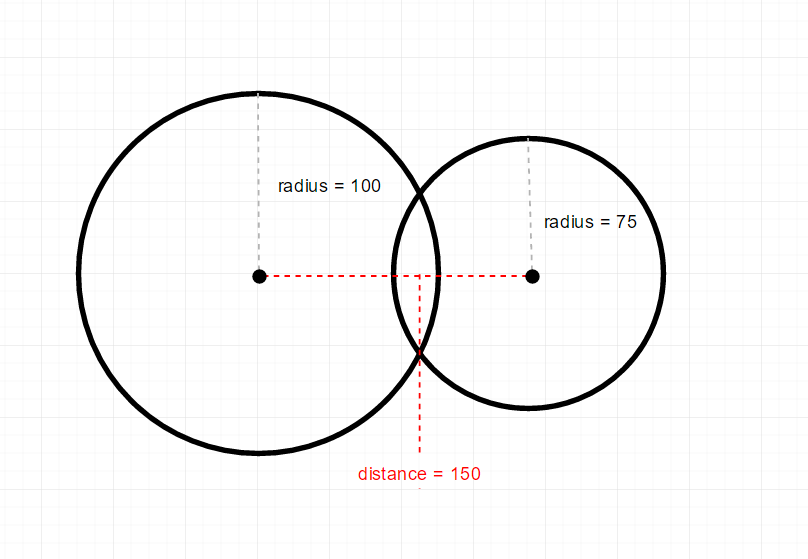
\includegraphics[width=0.8\textwidth]{collision-detection-6.png}  
	\caption{Kollision} 
	\label{Bild: Kollision}  
\end{figure}

\newpage

Die Formel zur Berechnung der Distanz zwischen den Punkten \( (x_1) \) und \( (x_2) \) lautet:

\[
\text{Abstand} = \sqrt{(x_2 - x_1)^2 + (y_2 - y_1)^2} [3]
\]

Im Code wird dies wie folgt umgesetzt:

\begin{verbatim}
	float dx = (float)(b1.sx - b2.sx);
	float dy = (float)(b1.sy - b2.sy);
	float distance = (float)Math.sqrt(dx * dx + dy * dy);
\end{verbatim}





\subsection{Impuls und Impulserhaltungssatz}

Impuls bezeichnet das Produkt aus der Masse eines Objekts und seiner Geschwindigkeit. Es handelt sich um eine Vektorgröße, die sowohl eine Richtung als auch eine Größe hat. Der Impuls eines Objekts bleibt nach einer elastischen Kollision erhalten, was bedeutet, dass die Gesamtimpulsmenge vor und nach der Kollision gleich bleibt.\\
Bei der Kollision zweier gleichmäßiger Objekte bleibt der Gesamtimpuls des Systems erhalten. Das bedeutet, dass die Summe der Impulse der beiden Objekte vor der Kollision gleich der Summe der Impulse nach der Kollision ist.\\
Wenn ein Objekt mit größerem Impuls auf ein Objekt mit kleinerem Impuls trifft, wird ein Teil des Impulses des ersten Objekts auf das zweite Objekt übertragen. Dies führt zu einer Änderung der Geschwindigkeiten beider Objekte, jedoch bleibt der Gesamtimpuls der Objekte unverändert.


	\vspace{0.5cm}

Die folgende Gleichung, bekannt als Impulserhaltungsgesetz stellt die Erhaltung der kinetischen Energie bei einem elastischen Stoß zwischen zwei Körpern dar.
		
		\[
		m_1 v_1^2 +  m_2 v_2^2 =  m_1 v_1'^2 +  m_2 v_2'^2
		\]
		
		\begin{itemize}
			\item \( m_1 \) und \( m_2 \) sind die Massen der Körper.
			\item \( v_1 \) und \( v_2 \) sind die Geschwindigkeiten der Körper vor dem Stoß.
			\item \( v_1' \) und \( v_2' \) sind die Geschwindigkeiten der Körper nach dem Stoß.
		\end{itemize}
		\vspace{0.5cm}
		
		
		Da wir nun wissen, dass der Gesamtimpuls der beiden objekten nach der Kollision gleich ist, können wir den Impuls, der zwischen den beiden Objekten während der Kollision übertragen wird, berechnen. Dazu berechnen wir zunächst das Skalarprodukt, das die relative Geschwindigkeit entlang der Kollisionsachse angibt. Wir teilen dieses Skalarprodukt durch die Summe der Massen der beiden Objekte, um den Impuls zu berechnen, der auf jedes Objekt übertragen wird. Dieser Impuls wird dann auf die Geschwindigkeiten der Objekte angewendet.
		
		 \[Skalararprodukt:
		\vec{a} \cdot \vec{b} = a_x b_x + a_y b_y 
		\]
		
Beispiel aus dem Code:

		\begin{verbatim}
			float nx = dx / distance;
			float ny = dy / distance;
			float dvx = (float)(b1.vx - b2.vx);
			float dvy = (float)(b1.vy - b2.vy);
			float skalarprodukt = dvx * nx + dvy * ny;
			
			if (skalarprodukt <= 0){
				
				float impuls = 2* skalarprodukt / (float)(b1.MASS + b2.MASS);
				
				b1.vx -= impuls * b2.MASS * nx;
				b1.vy -= impuls * b2.MASS * ny;
				b2.vx += impuls * b1.MASS * nx;
				b2.vy += impuls * b1.MASS * ny;
			};
		\end{verbatim}

		
		
		\subsection{Effet}
		
		Als Effet (franz. Wirkung) bezeichnet man den Drall eines Balls bzw. einer Kugel. [4] Es handelt sich um einen visuellen Effekt, mit dem man feststellen kann, dass sich ein Objekt dreht. Die Rotation des Balls ergibt sich aus seiner Geschwindigkeit und seinem Radius.
		
\[
\text{w} = \frac{\text{v}}{\text{r}} [5]
\]

		
		Im Code wird dies wie folgt umgesetzt:
		
		\begin{verbatim}
			cBalls.ball[i].angleX += cBalls.ball[i].vx * 0.1 / cBalls.ball[i].radius;
			cBalls.ball[i].angleY += cBalls.ball[i].vy * 0.1 / cBalls.ball[i].radius;
		\end{verbatim}
		
		
		Letzendlich muss der Winkel des Balls kontinuierlich angepasst werden. Dies erfolgt in Processing in der fortlaufenden \texttt{draw()} Methode:
		
		\begin{verbatim}
			public class Ball
			{..
			 void draw() {
				if (times >= 0) {
				..
					rotateX(angleX);     
					rotateY(angleY);      
					
				..
				}
			}..}
		\end{verbatim}
		
		Grundsätzlich sind die Sphären in Processing einfarbig. Im Rahmen dieser Veranstaltung haben wir eine weitere, kleinere Sphäre an den Koordinaten der ursprünglichen Sphäre positioniert, um das Drehmoment zu beobachten.		
		
		
	
	\section{Algorithmen zur Kollisionsdetektion}
	
	\subsection{Bruteforce}
	Vor- und Nachteile
	\subsection{Quad-Tree}
	Vorteile gegenüber Bruteforce
	
	\section{Visualisierungen und Demonstrationen}
	
	\subsection{Vektorenrichtung Drawer}
	
	\subsection{Tunneling-Demonstration}
	
	
	\subsection{Impuls-Demonstration}
	
	\subsection{Effet}
	
	\section{Fazit }
	
	\newpage
\begin{thebibliography}{5}
	\bibitem{leifiphysik}
	\href{https://www.leifiphysik.de/mechanik/impulserhaltung-und-stoesse/grundwissen/zentraler-elastischer-stoss}{Leifi Physik: Zentraler elastischer Stoß}
	\bibitem{happycoding}
	\href{https://happycoding.io/tutorials/processing/collision-detection}{Happy Coding: Collision Detection Tutorial}
	\bibitem{serlo}
	\href{https://de.serlo.org/mathe/1783/abstand-zweier-punkte-berechnen}{Serlo: Abstand zweier Punkte berechnen}
	\bibitem{Wiki}
	\href{https://de.wikipedia.org/wiki/Effet}{Effet - Wikipedia}
		\bibitem{leifiphysik}
	\href{	https://www.leifiphysik.de/mechanik/kreisbewegung/grundwissen/bahngeschwindigkeit-und-winkelgeschwindigkeit}{Bahngeschwindigkeit und Winkelgeschwindigkeit}

\end{thebibliography}

	
	
\end{document}










\end{document}
